\documentclass[border=10pt]{standalone}
\usepackage{tikz}\usepackage{amsmath}\usetikzlibrary{arrows.meta}
\begin{document}
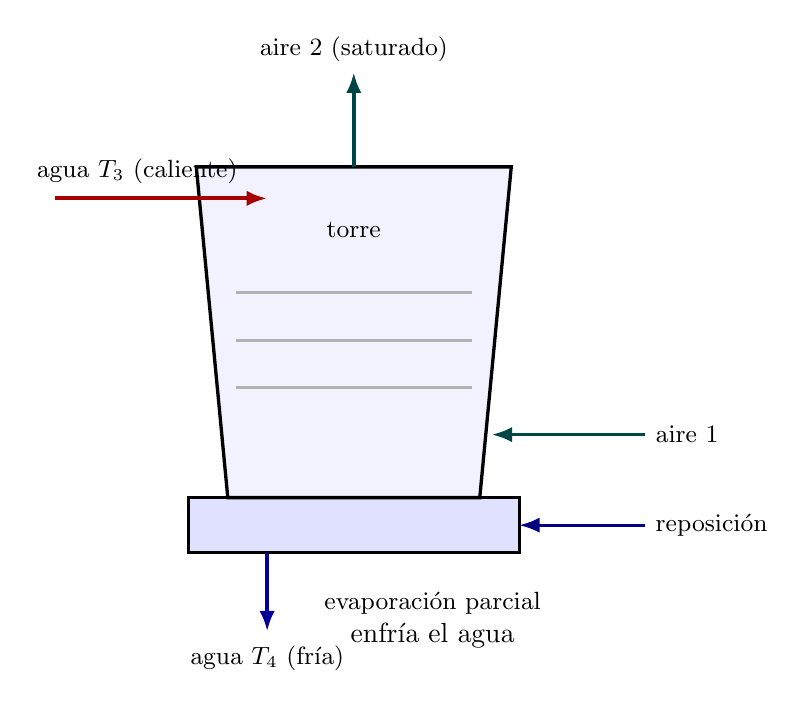
\begin{tikzpicture}[line width=1pt,>={Latex[length=2.6mm]}]
  % estanque (basin) inferior
  \fill[blue!12] (-0.1,-0.7) rectangle (4.1,0.0);
  \draw[line width=1.0pt] (-0.1,-0.7) rectangle (4.1,0.0);
  % torre (trapecio invertido ligero)
  \fill[blue!5] (0.4,0)--(3.6,0)--(4.0,4.2)--(0,4.2)--cycle;
  \draw[line width=1.2pt] (0.4,0)--(3.6,0)--(4.0,4.2)--(0,4.2)--cycle;
  % relleno (lineas)
  \foreach \y in {1.4,2.0,2.6} \draw[black!30] (0.5,\y)--(3.5,\y);
  \node at (2.0,3.4){\small torre};
  % agua caliente entra arriba (izquierda)
  \draw[->,red!65!black,line width=1.4pt] (-1.8,3.8)--(0.9,3.8);
  \node[above] at (-0.75,3.85){\small agua $T_3$ (caliente)};
  % aire sale arriba (saturado)
  \draw[->,teal!55!black,line width=1.3pt] (2.0,4.2)--(2.0,5.4);
  \node[above] at (2.0,5.4){\small aire 2 (saturado)};
  % aire entra abajo-derecha (dentro de la torre)
  \draw[->,teal!55!black,line width=1.3pt] (5.7,0.8)--(3.75,0.8);
  \node[right] at (5.7,0.8){\small aire 1};
  % reposicion entra al estanque por la derecha (mas abajo que el aire)
  \draw[->,blue!50!black,line width=1.1pt] (5.7,-0.35)--(4.1,-0.35);
  \node[right] at (5.7,-0.35){\small reposición};
  % agua fria sale por abajo-izquierda del estanque
  \draw[->,blue!60!black,line width=1.4pt] (0.9,-0.7)--(0.9,-1.7);
  \node[below] at (0.9,-1.75){\small agua $T_4$ (fría)};
  % nota inferior
  \node[align=center] at (3.0,-1.55){\small evaporación parcial\\ enfría el agua};
\end{tikzpicture}
\end{document}
